% Estimating viewpoint continuously to fine tune a initial matching
The NZ-WHO template matching method we have presented
(Sect.~\ref{sec:nzwho}) makes template generation and evaluation
computationally inexpensive. This means that we can use a
hypothesize-and-test scheme to efficiently explore the continuous
parameter space to find the best object pose, scale, 3D CAD model type
and camera focal length.
%
In particular, we propose to implement this parameter search as a
Markov Chain Monte Carlo (MCMC) procedure based on the
Metropolis-Hastings algorithm.

\paragraph{Probabilistic formulation.}
We parameterize the continuous parameter space as  $x = [p, m, f]$,
where $p$ is the 3D rotation of the CAD model, $m$ is the discrete CAD
model index, and $f$ is the focal length.

We model the probability that the object in the test image
$\mathcal{I}$ is generated by the parameters $x$ as a distribution in
the exponential family, and let
\begin{align}
    P(x) & \sim e^{ c_4 \max_{s} w(x) \ast \mathcal{T}_s(\mathcal{I})},
\end{align}
where $\max_{s} w(x) \ast T(\mathcal{I})$ is the convolution score of
template $w(x)$ with image feautures $T(\mathcal{I})$, as defined
in Sect.~\ref{}.

\paragraph{Inference.}
We approximate the MAP solution for $x$ by drawing samples from the
distribution $P(x)$, using the Metropolis-Hastings
algorithm. Specifically, we use a variant that changes only a single
component of the parameter vector $x$ at a time, termed Single
Component Metropolis Hastings.

This algorithm changes the current state $x$ to a new state $x'$ based
on the acceptance probability
\begin{align}
    A(x \rightarrow x') & =  min\left( 1,  \frac{P(x' g(x') \rightarrow x)}{P(x) g(x \rightarrow x')}\right).
\end{align}
We define $4$ different types of moves that can alter the state
(Fig.~\ref{fig:moves}), {\em (i)} changing the focal length $f$, {\em
  (ii)} one of the rotational pose parameters $p_i$, {\em (iii)} scale
  or translation, and {\em (iv)} CAD model index $m$. For (i) to
  (iii), we use Gaussian proposal distributions, and a uniform
  distribution over model changes for (iv).
\begin{align}
    g(x \rightarrow x + p_i') & \sim \mathcal{N}(\mu = 0,\sigma = c_1) \quad i \in \{1,2,3\}\\
    g(x \rightarrow x + f') & \sim \mathcal{N}(\mu = 0,\sigma = c_2)\\
    g(x \rightarrow x + m') & \sim c_3 \delta(m) + (1-c_3) Unif(1,M),
\end{align}
where $g$ is the proposal distribution. % and $P$ is the distribution of which we
%defined using Gaussian distribution around previous state. $A$ is the
%acceptance probability where we accept new proposal with $A(x \rightarrow x')$.
%
% One can also think of the image as an image cropped by detection
% bounding box. We synthesize covariance matrix and create NZ-WHO
% template $w(x)$ for particular viewpoint, focal length and CAD model.
% In sum, for new proposal $x'$, we make a NZ-WHO template on the fly 
% We found out that it requires good initialization to converge to
% local minima.
In practice, we run this algorithm for \scream{} iterations, keeping
the sample with the highest probability as our approximate estimate of
the MAP solution.
\scream{no idea what c is}


% there are several advantages that was not possible such as
% \textbf{on-the-fly} template generation and making large number of
% templates
\begin{figure}[t]
\centering
    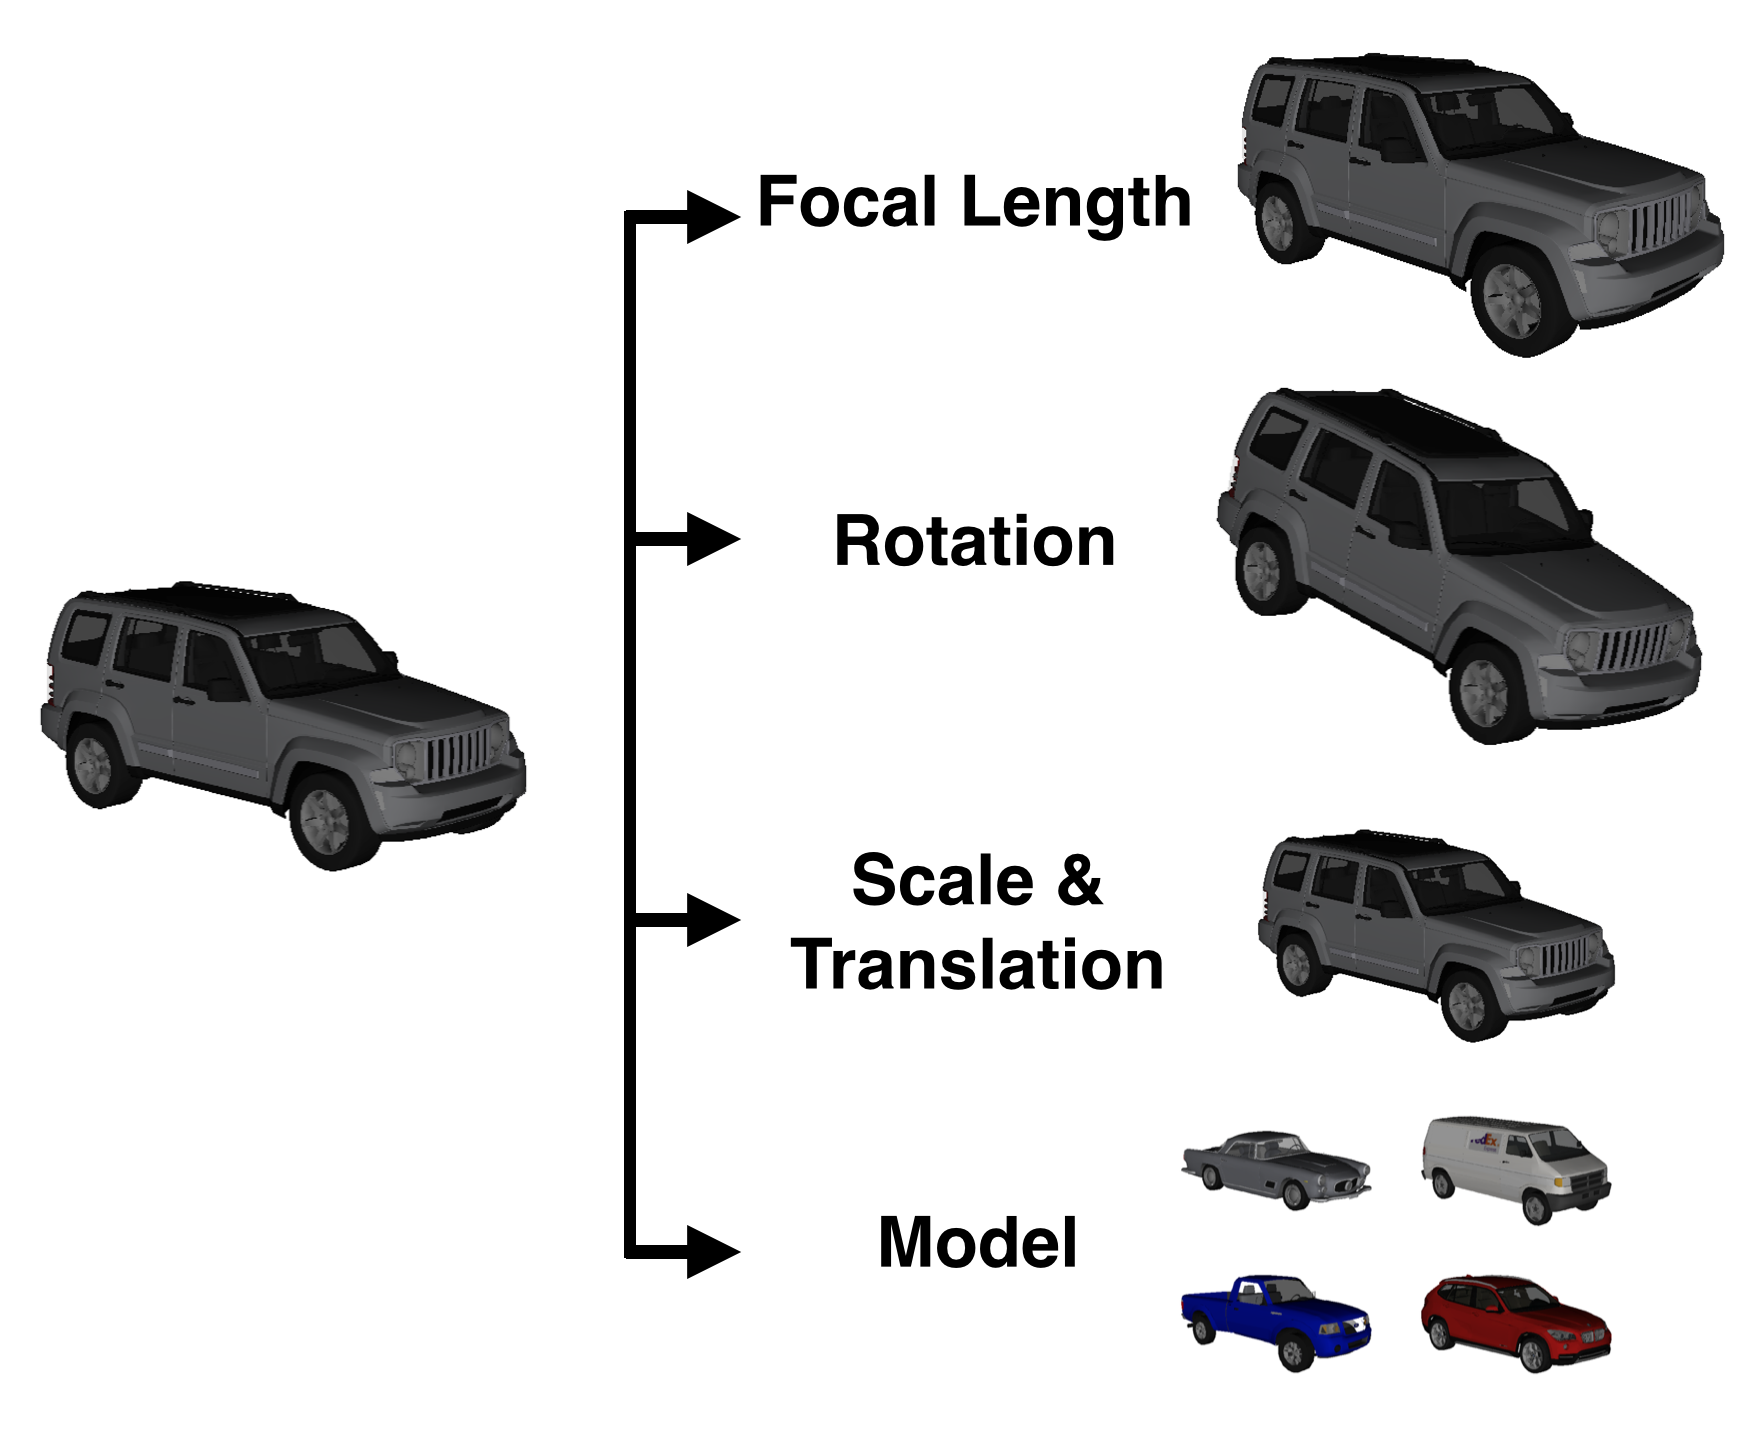
\includegraphics[width=0.7\linewidth]{tuning2} \\ [-5pt]
    \caption{Metropolis Hastings move types (Section~\ref{sec:fine}).}
 \label{fig:moves}
\end{figure}


\paragraph{Initialization.}
Since the Metropolis-Hastings algorithm is susceptible to getting
stuck in local optima, we need a good initialiation in order to
increase the probability to find a solution that is close to the
global optima. We achieve this by first running a discrete,
pre-trained version of our algorithm (i.e., an ensemble of NZ-WHO
templates) in order to get promising candidate 2D bounding boxes and
poses to start from. We then initialize $x_0$ for each of these candidates.
